\renewcommand*{\arraystretch}{1.1}

\label{sec:interactive-short-read-01}
\noindent\begin{tabularx}{\queryCardWidth}{|>{\queryPropertyCell}c|X|}
	\hline
	query & Interactive / short / 1 \\ \hline
%
	title & Person Profile \\ \hline
%
    pattern & \hfill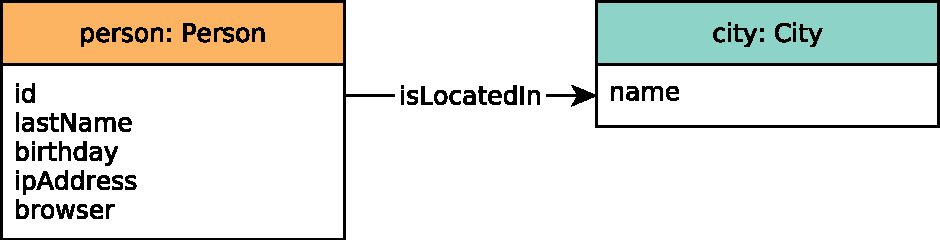
\includegraphics[scale=\patternscale,margin=0cm .2cm]{patterns/interactive-short-read-01}\hfill\vadjust{} \\ \hline
%
	desc. & Given a start Person, retrieve their first name, last name, birthday, IP
address, browser, and city of residence.
 \\ \hline
%
	
%
    
        params &
        \innerCardVSpace{\begin{tabularx}{\attributeCardWidth}{|>{\paramNumberCell}c|>{\varNameCell}M|>{\typeCell}m{\typeWidth}|Y|} \hline
        \cellcolor{parameter} \color{white} \footnotesize $\mathsf{1}$ &Person.id& ID &  \\ \hline
        \end{tabularx}}\innerCardVSpace \\ \hline
	
%
	
        result &
        \innerCardVSpace{\begin{tabularx}{\attributeCardWidth}{|>{\resultNumberCell}c|>{\varNameCell}M|>{\typeCell}m{\typeWidth}|>{\resultOriginCell}c|Y|} \hline
        $\mathsf{1}$ & Person.firstName & String &R&
                 \\ \hline
        $\mathsf{2}$ & Person.lastName & String &R&
                 \\ \hline
        $\mathsf{3}$ & Person.birthDay & Date &R&
                 \\ \hline
        $\mathsf{4}$ & Person.locationIP & String &R&
                 \\ \hline
        $\mathsf{5}$ & Person.browserUsed & String &R&
                 \\ \hline
        $\mathsf{6}$ & Person-isLocatedIn->Place.id & 32-bit Integer &R&
                 \\ \hline
        $\mathsf{7}$ & Person.gender & String &R&
                 \\ \hline
        $\mathsf{8}$ & Person.creationDate & DateTime &R&
                 \\ \hline
        \end{tabularx}}\innerCardVSpace \\ \hline
	
%
	%
	%
	%
    %
\end{tabularx}
\queryCardVSpace